\documentclass[a4paper]{article}
\usepackage[utf8]{inputenc}
\usepackage{amsthm, amsmath, mathtools, amssymb}
\usepackage[left=2cm,right=2cm,top=2cm,bottom=2cm]{geometry}
\usepackage[colorlinks,linkcolor=blue,citecolor=blue,urlcolor=blue]{hyperref}
\usepackage{array}
\usepackage[catalan,english]{babel}
\usepackage[affil-it]{authblk}
\usepackage{titlesec}
\usepackage[intlimits]{esint} % for more options on integrals.
\usepackage{physics}
\usepackage[hypcap=false]{caption}
\usepackage{subcaption}
\usepackage{multirow}
% \titleformat{\section}
%   {\normalfont\fontsize{13}{15}\bfseries}{\thesection}{1em}{}

\newcommand{\NN}{\ensuremath{\mathbb{N}}} % set of natural numbers
\newcommand{\ZZ}{\ensuremath{\mathbb{Z}}} % set of integers
\newcommand{\QQ}{\ensuremath{\mathbb{Q}}} % set of rationals
\newcommand{\RR}{\ensuremath{\mathbb{R}}} % set of real numbers
\newcommand{\CC}{\ensuremath{\mathbb{C}}} % set of complex numbers
\newcommand{\KK}{\ensuremath{\mathbb{K}}} % a general field

\newcommand{\vf}[1]{\boldsymbol{\mathrm{#1}}} % math style for vectors and matrices and vector-values functions (previously it was \*vb{#1} but this does not apply to greek letters)
\newcommand{\ii}{\mathrm{i}} % imaginary unit
\newtheorem{theorem}{Teorema}
\newtheorem{prop}{Proposició}
\theoremstyle{definition}
\newtheorem{definition}{Definició}
\DeclareDocumentCommand\derivative{ s o m g d() }{ 
  % Total derivative
  % s: star for \flatfrac flat derivative
  % o: optional n for nth derivative
  % m: mandatory (x in df/dx)
  % g: optional (f in df/dx)
  % d: long-form d/dx(...)
    \IfBooleanTF{#1}
    {\let\fractype\flatfrac}
    {\let\fractype\frac}
    \IfNoValueTF{#4}
    {
        \IfNoValueTF{#5}
        {\fractype{\diffd \IfNoValueTF{#2}{}{^{#2}}}{\diffd #3\IfNoValueTF{#2}{}{^{#2}}}}
        {\fractype{\diffd \IfNoValueTF{#2}{}{^{#2}}}{\diffd #3\IfNoValueTF{#2}{}{^{#2}}} \argopen(#5\argclose)}
    }
    {\fractype{\diffd \IfNoValueTF{#2}{}{^{#2}} #3}{\diffd #4\IfNoValueTF{#2}{}{^{#2}}}\IfValueT{#5}{(#5)}}
} % differential operator
\DeclareDocumentCommand\partialderivative{ s o m g d() }{ 
  % Total derivative
  % s: star for \flatfrac flat derivative
  % o: optional n for nth derivative
  % m: mandatory (x in df/dx)
  % g: optional (f in df/dx)
  % d: long-form d/dx(...)
  \IfBooleanTF{#1}
    {\let\fractype\flatfrac}
    {\let\fractype\frac}
    \IfNoValueTF{#4}{
      \IfNoValueTF{#5}
      {\fractype{\partial \IfNoValueTF{#2}{}{^{#2}}}{\partial #3\IfNoValueTF{#2}{}{^{#2}}}}
      {\fractype{\partial \IfNoValueTF{#2}{}{^{#2}}}{\partial #3\IfNoValueTF{#2}{}{^{#2}}} \argopen(#5\argclose)}
    }
    {\fractype{\partial \IfNoValueTF{#2}{}{^{#2}} #3}{\partial #4\IfNoValueTF{#2}{}{^{#2}}}\IfValueT{#5}{(#5)}}
} % partial differential operator

\renewcommand{\labelenumii}{\alph{enumii})}

\title{\bfseries\large SEMINARI 2\\\vspace{0.25cm}Problema centre - focus i bifurcació de Hopf}

\author{Víctor Ballester Ribó\endgraf NIU:1570866}
\date{\parbox{\linewidth}{\centering
  Sistemes dinàmics\endgraf
  Grau en Matemàtiques\endgraf
  Universitat Autònoma de Barcelona\endgraf
  Gener de 2023}}

\setlength{\parindent}{0pt}
\begin{document}
\selectlanguage{catalan}
\maketitle
En aquest document ens dedicarem a estudiar l'estabilitat de l'origen en funció de paràmetres per a diferents sistemes diferencials així com el nombre d'òrbites periòdiques que poden néixer de l'origen en cada cas.
\section*{Exercici 1}
Considerem el sistema diferencial:
\begin{equation}\label{sis1}
  \left\{
  \begin{aligned}
    x' & =-y                    \\
    y' & =x + ay +bx^2+cx^3+x^4
  \end{aligned}
  \right.
\end{equation}
amb $a,b,c\in\RR$.

Observem d'entrada que si $a\ne 0$, l'origen és hiperbòlic i per tant és estable si $a<0$ i inestable si $a>0$. Pel cas $a=0$, fixem-nos que el sistema és Hamiltonià amb integral primera (definida en un entorn de l'origen): $$H=\frac{x^2}{2}+\frac{y^2}{2}+b\frac{x^3}{3}+c\frac{x^4}{4}+\frac{x^5}{5}$$
Per tant, com que el sistema rota al voltant de l'origen, aquest és un centre $\forall b,c \in\RR$.

Finalment notem que la divergència del sistema és $a$. I per tant si $a\ne 0$, el teorema de Bendixson ens assegura que no hi ha cicles límit al sistema per cap valor de $a,b,c\in\RR$, $a\ne 0$.
\section*{Exercici 2}
Considerem el sistema diferencial:
\begin{equation}\label{sis2}
  \left\{
  \begin{aligned}
    x' & =ax-y+x^2     \\
    y' & =x + y^2+b xy
  \end{aligned}
  \right.
\end{equation}
amb $a,b\in\RR$.

El sistema té divergència $a+2x+2y+bx$, que té signe constant en un entorn de l'origen si $a\ne 0$. Per tant, l'estabilitat de l'origen si $a\ne 0$ ve donada pel signe de $a$. Quan $a>0$, l'origen és inestable; quan $a<0$, és estable. Ara suposem $a=0$. La primera constant de Lyapunov és $L_1=-b/4$. Per tant, aquest cop l'estabilitat ve donada pel signe de $b$. Si ara suposem $a=b=0$, el sistema resultant
$$
  \left\{
  \begin{aligned}
    x' & =-y+x^2  \\
    y' & =x + y^2
  \end{aligned}
  \right.
$$
és simètric respecte el canvi $(x, y, t)\to(-y,-x,-t)$, que correspon a la simetria respecte la recta $x+y=0$. Com que el sistema rota en un entorn de l'origen, aquest és un centre. En resum, em obtingut els següents resultats:
$$\text{L'origen és un }
  \begin{cases}
    \text{focus estable}   & \text{si } a < 0 \text{ o } a = 0, b>0  \\
    \text{focus inestable} & \text{si } a > 0  \text{ o } a = 0, b<0 \\
    \text{centre}          & \text{si } a = b= 0
  \end{cases}
$$
Per estudiar el nombre de cicles límit que neixen de l'origen fixem-nos que si $a=0$, podem escriure la funció de retorn en sèrie de potències respecte $L_1$ i factoritzar-la de la forma:
$$\Delta (\rho)=L_1\rho^3(1 + \mathrm{O}(\rho^2))$$
que és un polinomi que no té zeros per $\rho\gtrsim 0$ i $b\ne 0$. Per tant, només tindrem un únic cicle límit bifurcant de l'origen, que és el corresponent a la traça.
\begin{figure}[ht]
  \centering
  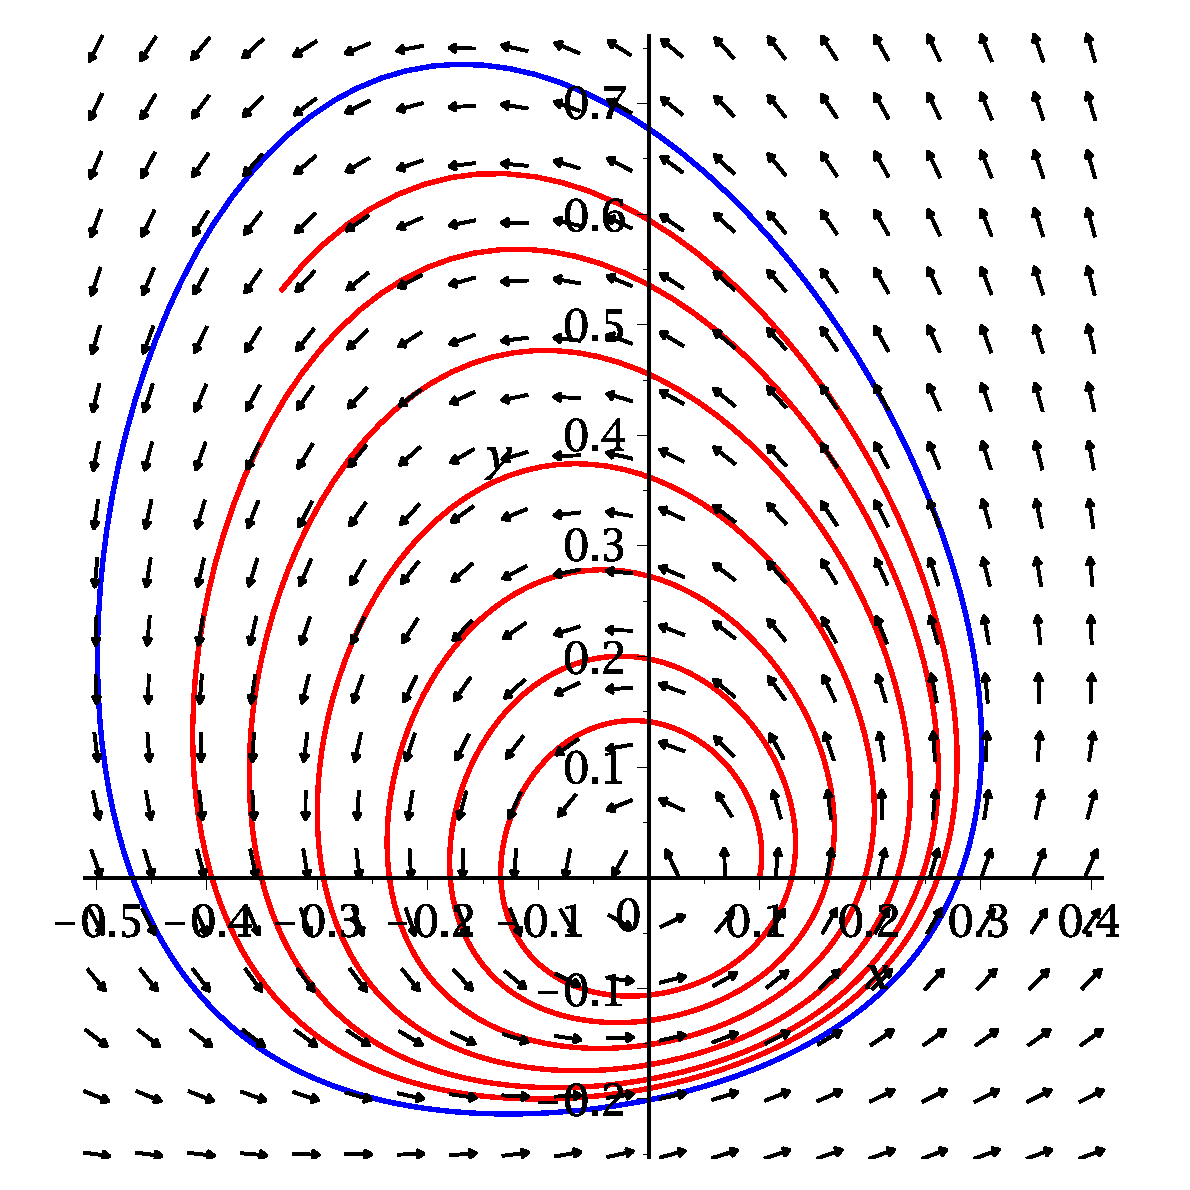
\includegraphics[width=0.5\linewidth]{Images/ex2-lc.eps}
  \caption{Cicle límit de Hopf del sistema \eqref{sis2} amb $a=0.1$ i $b=3$}
\end{figure}
\section*{Exercici 3}
Considerem el sistema diferencial:
\begin{equation}\label{sis3}
  \left\{
  \begin{aligned}
    x' & =-y+xy+x^2      \\
    y' & =x + ax^2 +by^2
  \end{aligned}
  \right.
\end{equation}
amb $a,b\in\RR$.

Les tres primeres constants de Lyapunov d'aquest sistema són les següents:
$$L_1=\frac{1-2a}{4}\qquad L_2=\frac{4b^3-7b-1}{16}\qquad L_3 = 0$$
on per calcular cadascuna, hem assumit que les anteriors eren zero. Recordem que, com que el sistema és quadràtic, no cal calcular-ne més, ja que totes les següents també seran 0. L'estabilitat, doncs, la tenim determinada excepte per quan $a=1/2$ i $b$ satisfà $4b^3-7b-1=0$. Les arrels d'aquest polinomi s'exposen a continuació: $$-0.1445842733...\quad -1.244644286...\quad 1.389228559...$$

Observem que per $a=1/2$ i $b$ proper
\section*{Exercici 4}
Considerem el sistema diferencial:
\begin{equation}\label{sis4}
  \left\{
  \begin{aligned}
    x' & =ax-y-9x^2+4xy+by^2   \\
    y' & =x +ay+2x^2-7xy -2y^2
  \end{aligned}
  \right.
\end{equation}
amb $a,b\in\RR$.


\section*{Exercici 5}
Considerem el sistema diferencial:
\begin{equation}\label{sis5}
  \left\{
  \begin{aligned}
    x' & = 6\varepsilon x-24ax^2-18xy-3\varepsilon+24x \\
    y' & =2(3y-2)(3y+\varepsilon)
  \end{aligned}
  \right.
\end{equation}
amb $a>0$ i $\varepsilon\in\RR$. En aquest cas se'ns demana estudiar l'estabilitat de tots els equilibris.

Els equilibris que tenim són els següents:
$$z_\pm^1= \left(\frac{\varepsilon+2\pm\sqrt{-8a\varepsilon+{(\varepsilon+2)}^2}}{8a},\frac{2}{3}\right) \quad z_\pm^2= \left(\frac{\varepsilon+2\pm\sqrt{-2a\varepsilon+{(\varepsilon+2)}^2}}{4a},-\frac{\varepsilon}{3}\right)$$
Els valors propis de les diferencials a cada punt són els següents:
\begin{align*}
  \sigma(DX(z_\pm^1)) & =\left\{12+6\varepsilon, \mp6\sqrt{-8a\varepsilon+{(\varepsilon+2)}^2}\right\}     \\
  \sigma(DX(z_\pm^2)) & =\left\{-(12+6\varepsilon), \mp12\sqrt{-2a\varepsilon+{(\varepsilon+2)}^2}\right\}
\end{align*}
Definim $f(a, \varepsilon)=-8a\varepsilon+{(\varepsilon+2)}^2$ i $g(a, \varepsilon) =-2a\varepsilon+{(\varepsilon+2)}^2$. Fixem-nos quan $f(a, \varepsilon)< 0$ perdrem dos punts d'equilibri i el mateix passa per $g(a,\varepsilon)$.
\begin{figure}[ht]
  \centering
  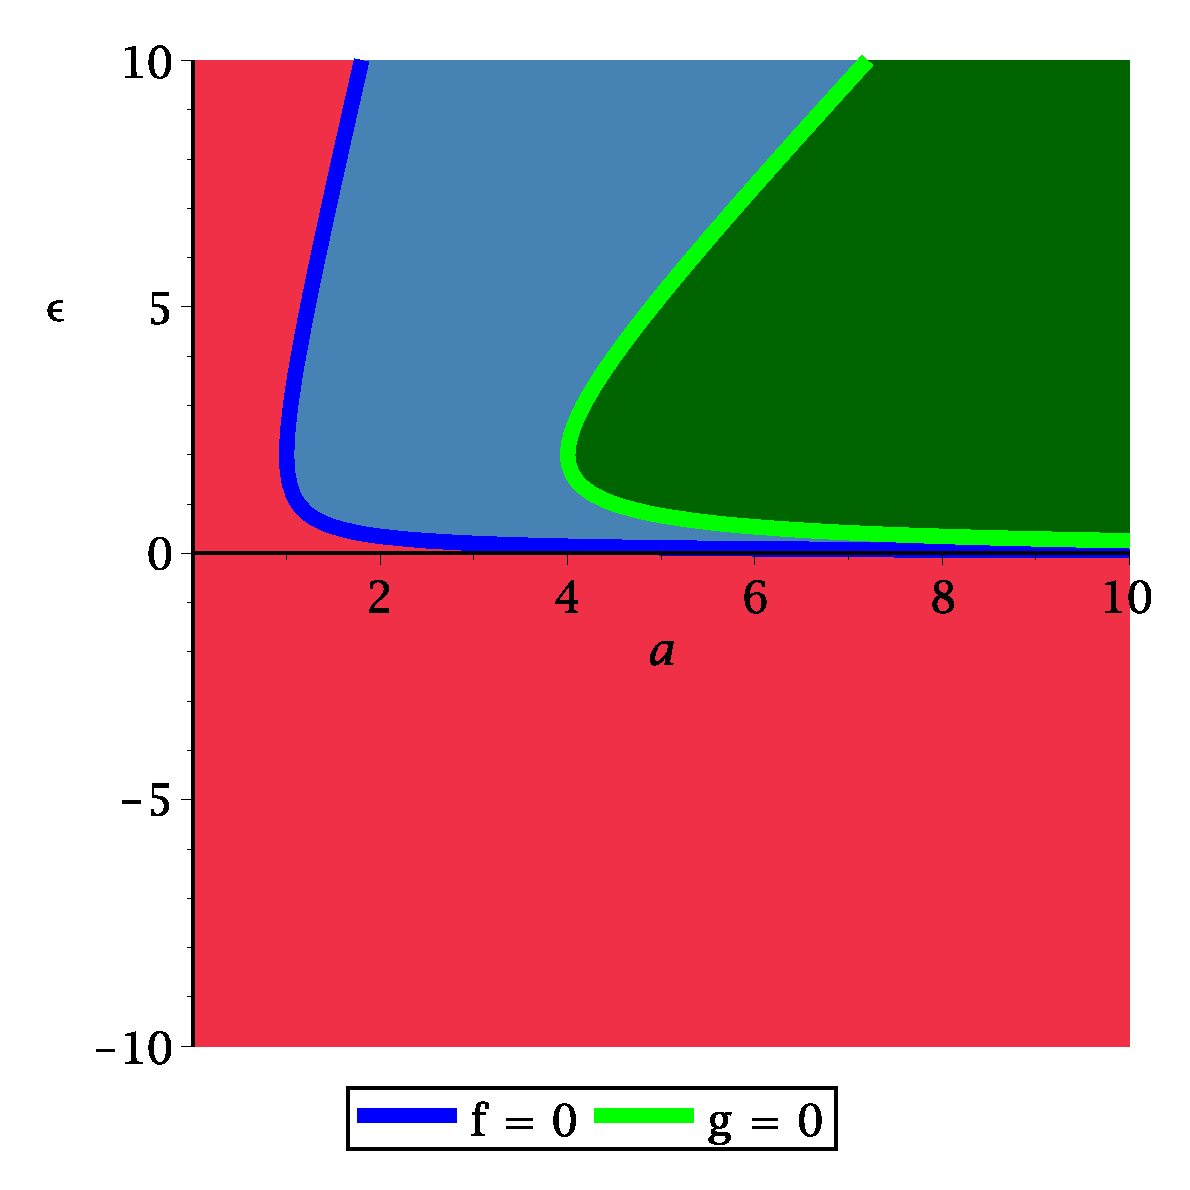
\includegraphics[width=0.5\linewidth]{Images/ex5-fg.eps}
  \caption{Gràfiques de les equacions $f=0$ i $g=0$}
  \label{ex5fg}
\end{figure}
Com podem observar a la figura \ref{ex5fg}, en la regió vermella tenim 4 punts crítics, en la regió blava 2 i en la verda 0. En les corbes blava i verda, tenim 3 i 1 equilibris respectivament.

En la regió vermella, els equilibris si $\varepsilon>-2$, $z_-^1$ i $z_+^2$ són selles i $z_+^1$ i $z_-^2$ nodes (inestable i estable, respectivament). Si $\varepsilon<-2$, $z_+^1$ i $z_-^2$ són selles i $z_-^1$ i $z_+^2$ nodes (estable i inestable, respectivament). Per $\varepsilon = -2$, $z_+^1=z_+^2=(\frac{1}{2\sqrt{a}},\frac{2}{3})$ i $z_-^1=z_-^2=(-\frac{1}{2\sqrt{a}},\frac{2}{3})$ amb valors propis $\{0,\mp 24\sqrt{a}\}$. Una de les dues varietats és atractora per un punt, i repulsora per a l'altre. Estudiant el camp sobre la varietat central, veiem que en ambdós casos comença amb sèrie amb $128a^2 z^2+\cdots$ (un cop havent centrat el punt a l'origen, és a dir $z\simeq 0)$. Per tant, tenim en ambdós casos un sella-node.

En la regió blava, l'estabilitat dels punts $z_\pm^2$ és la mateixa que en la regió vermella quan $\varepsilon > -2$. Finalment en les dues corbes $f=0$ i $g=0$, on els punts co\lgem isonen, tenim en ambdós casos un valor propi 0 i estudiant el camp sobre la seva corresponent varietat central deduïm que són selles nodes.

A continuació presentem els diagrames de bifurcació per a diverses seccions $a=\mathrm{const}$. En els següents gràfics la línia contínua representa el punt $z_+^1$; la discontínua amb punts, el punt $z_-^1$; la discontínua amb ratlles, el punt $z_+^2$, i la discontínua amb punts i ratlles, el punt $z_-^2$.

\begin{figure}[ht]
  \captionsetup[subfigure]{justification=centering}
  \centering
  \begin{subfigure}[b]{0.4\linewidth}
    \centering
    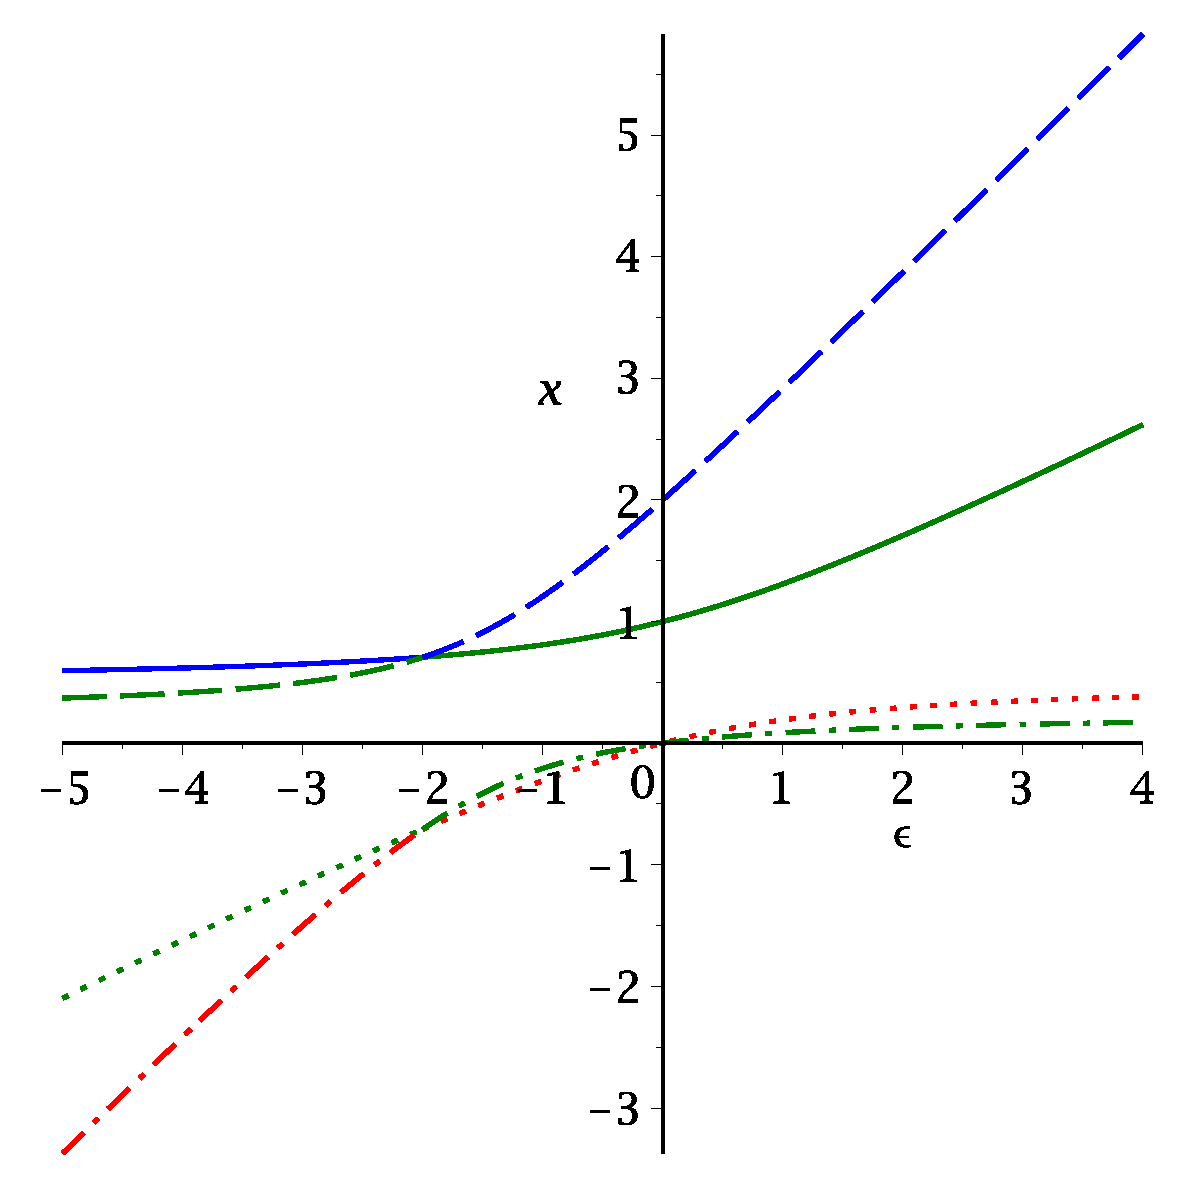
\includegraphics[width=\linewidth]{Images/ex5-a05x.eps}
    \caption{Gràfic $\varepsilon - x$}
  \end{subfigure}
  \hfill
  \begin{subfigure}[b]{0.4\linewidth}
    \centering
    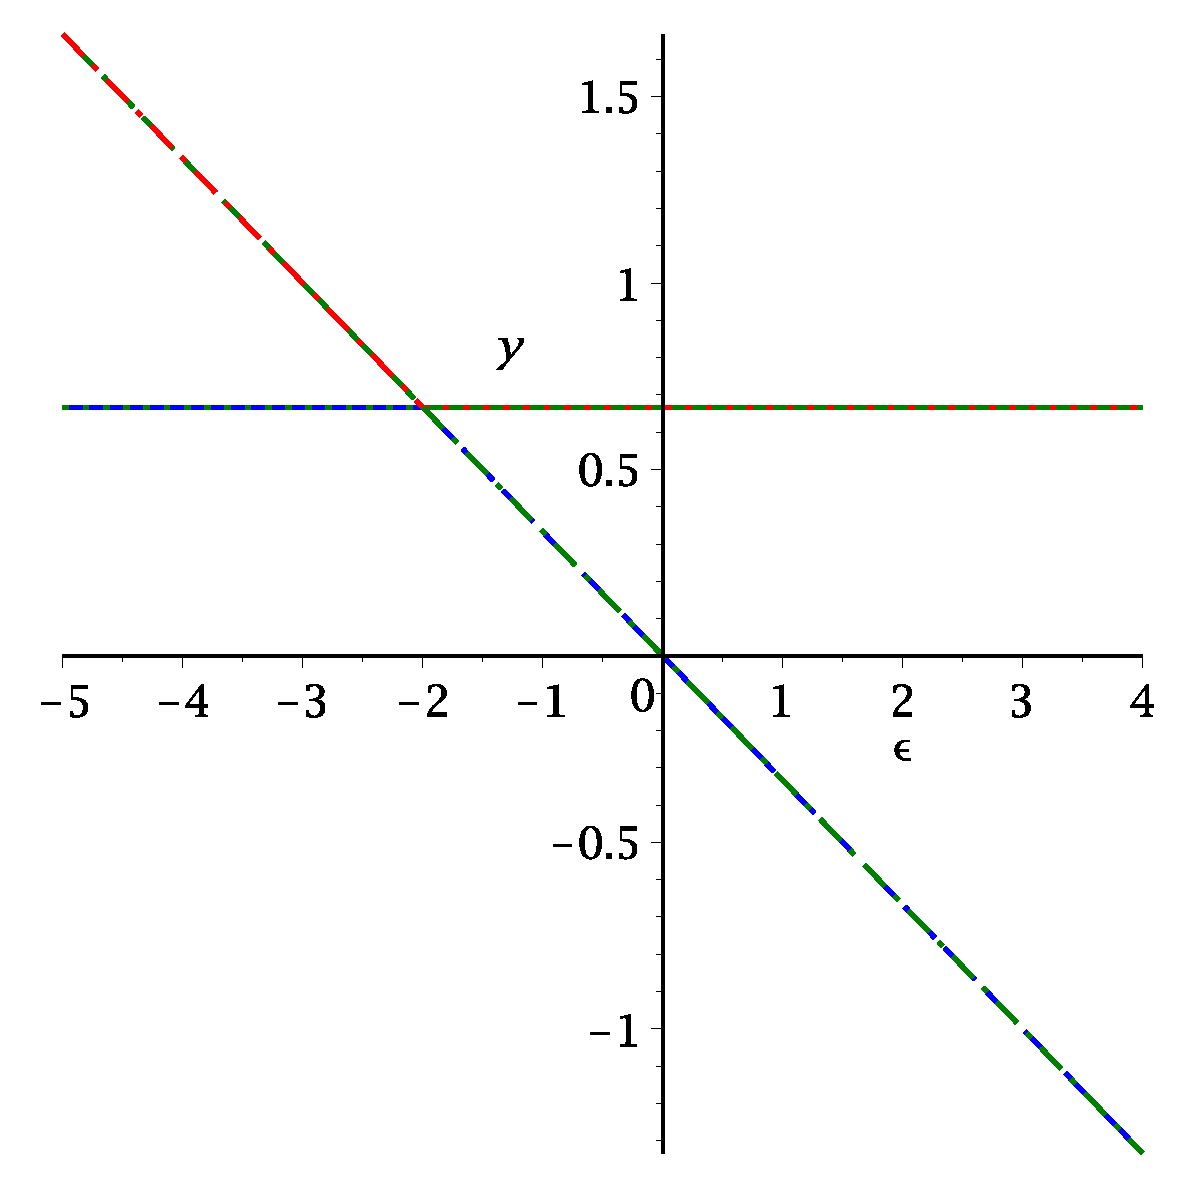
\includegraphics[width=\linewidth]{Images/ex5-a05y.eps}
    \caption{Gràfic $\varepsilon - y$}
  \end{subfigure}
  \caption{Diagrama de bifurcació dels punts d'equilibri quan $a=1/2$}
\end{figure}

Pels següents gràfics ometrem el diagrama de les $y$, ja que sempre és de la mateixa forma.

\begin{figure}[ht]
  \captionsetup[subfigure]{justification=centering}
  \centering
  \begin{subfigure}[b]{0.4\linewidth}
    \centering
    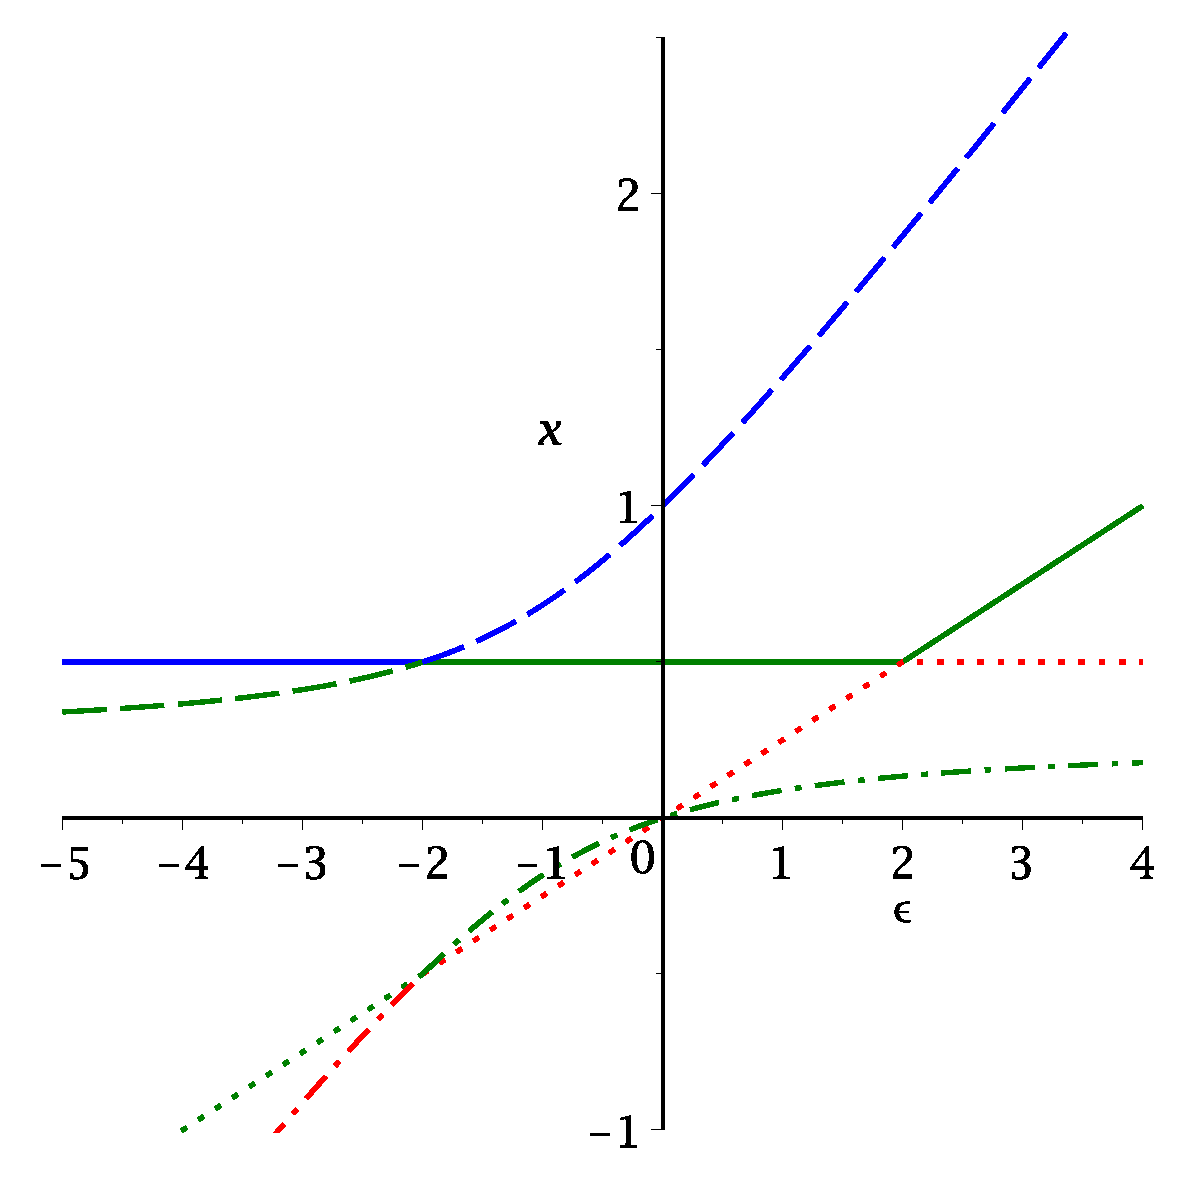
\includegraphics[width=\linewidth]{Images/ex5-a1.eps}
    \caption{Diagrama de bifurcació dels punts d'equilibri quan $a=1$}
  \end{subfigure}
  \hfill
  \begin{subfigure}[b]{0.4\linewidth}
    \centering
    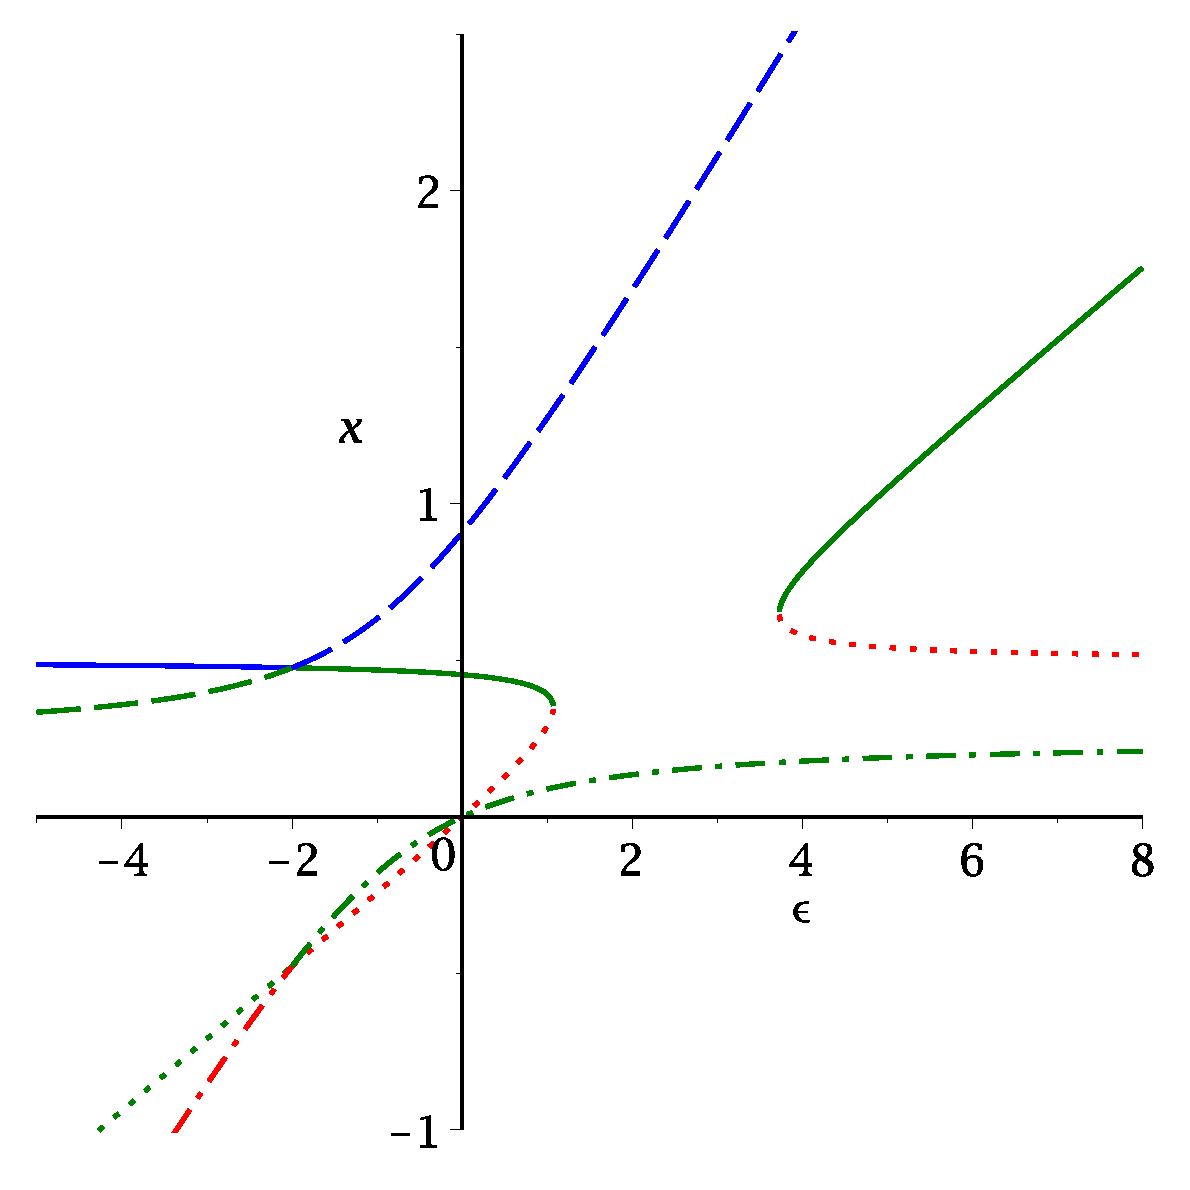
\includegraphics[width=\linewidth]{Images/ex5-a2.eps}
    \caption{Diagrama de bifurcació dels punts d'equilibri quan $a=2$}
    \label{fig2}
  \end{subfigure}
  \\
  \centering
  \begin{subfigure}[b]{0.4\linewidth}
    \centering
    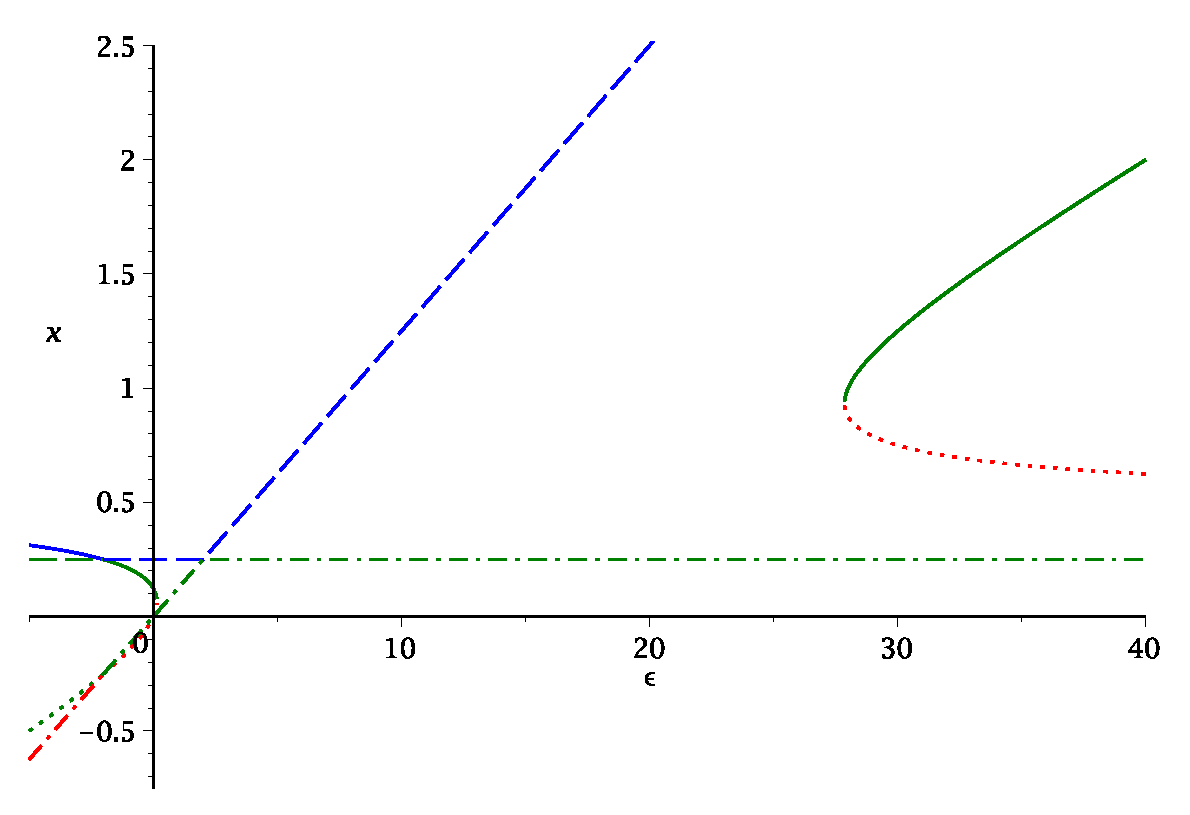
\includegraphics[width=\linewidth]{Images/ex5-a4.eps}
    \caption{Diagrama de bifurcació dels punts d'equilibri quan $a=4$}
  \end{subfigure}
  \hfill
  \begin{subfigure}[b]{0.4\linewidth}
    \centering
    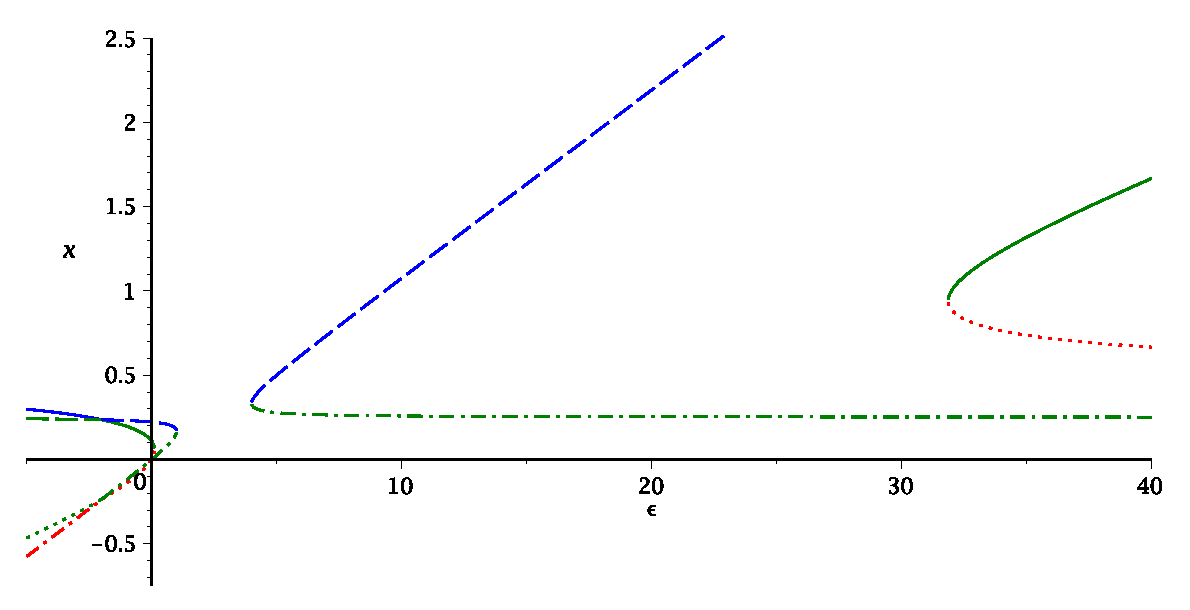
\includegraphics[width=\linewidth]{Images/ex5-a45.eps}
    \caption{Diagrama de bifurcació dels punts d'equilibri quan $a=4.5$}
  \end{subfigure}
\end{figure}
\section*{Exercici 6}
Considerem el sistema diferencial:
\begin{equation}\label{sis6}
  \left\{
  \begin{aligned}
    x' & =y                & =:  f_1(x,y) \\
    y' & =-x + \mu(1-x^2)y & =: f_2(x,y)
  \end{aligned}
  \right.
\end{equation}
amb $a,b,c\in\RR$. Volem estudiar l'estabilitat de l'origen en funció de $a$, $b$ i $c$ així com el nombre d'òrbites periòdiques que poden néixer d'aquest.
\section*{Exercici 7}
Considerem el sistema diferencial:
\begin{equation}\label{sis7}
  \left\{
  \begin{aligned}
    x' & =y                          \\
    y' & =\beta_1+\beta_2x + x^2 +xy
  \end{aligned}
  \right.
\end{equation}
amb $\beta_1,\beta_2\in\RR$. Se'ns demana estudiar quan obtindrem una bifurcació de Hopf. Per això estaria bé conèixer l'estabilitat dels equilibris segons $\beta_1$ i $\beta_2$.

Suposem d'entrada ${\beta_2}^2\geq 4\beta_1$, perquè si no el sistema no té equilibris. En aquest cas, aquests juntament amb els seus valors propis són els següents:
\begin{align*}
  z_+ & =\left(-\frac{\beta_2}{2}+\frac{\sqrt{{\beta_2}^2-4\beta_1}}{2},0\right)\quad \sigma(D\vf{X}(z_+))=\left\{-\frac{\beta_2}{2}+\frac{\sqrt{{\beta_2}^2-4\beta_1}}{2}\pm\frac{\sqrt{f(\beta_1,\beta_2)}}{4}\right\} \\
  z_- & =\left(-\frac{\beta_2}{2}-\frac{\sqrt{{\beta_2}^2-4\beta_1}}{2},0\right)\quad \sigma(D\vf{X}(z_-))=\left\{-\frac{\beta_2}{2}-\frac{\sqrt{{\beta_2}^2-4\beta_1}}{2}\pm\frac{\sqrt{g(\beta_1,\beta_2)}}{4}\right\}
\end{align*}
on:
\begin{align*}
  f(\beta_1,\beta_2)=2{\beta_2}^2-4\beta_1-2\beta_2\sqrt{{\beta_2}^2-4\beta_1}+16\sqrt{{\beta_2}^2-4\beta_1} \\
  g(\beta_1,\beta_2)=2{\beta_2}^2-4\beta_1+2\beta_2\sqrt{{\beta_2}^2-4\beta_1}-16\sqrt{{\beta_2}^2-4\beta_1}
\end{align*}

Comencem l'estudi suposant que els dos punts són iguals, és a dir que ${\beta_2}^2=4\beta_1$. Si $\beta_2=\beta_1=0$, l'origen és un \emph{cusp}, pel teorema de classificació de punts nilpotents. Ara suposem $\beta_2\ne 0$ i passem el sistema a la seva forma de Jordan:
\begin{equation}
  \left\{
  \begin{aligned}
    x' & =X(x,y,\vf\beta)                     \\
    y' & =-\frac{\beta_2}{2}y+Y(x,y,\vf\beta)
  \end{aligned}
  \right.
\end{equation}
on $\vf\beta=(\beta_1,\beta_2)$ i $X$ i $Y$ tenen sèrie de Taylor començant per ordre 2. Fent càlculs i usant el teorema de classificació de punts semihiperbòlics resulta que obtenim un sella-node.

Ara suposem que ${\beta_2}^2>4\beta_1$ i observem que: $$f(\beta_1,\beta_2)={\left(\beta_2-\sqrt{{\beta_2}^2-4\beta_1}\right)}^2+16\sqrt{{\beta_2}^2-4\beta_1}> 0$$
Per tant, $z_+$ sempre té valors propis reals i el seu producte és $-\sqrt{{\beta_2}^2-4\beta_1}< 0$. Per tant, aquest punt sempre és una sella.

Centrem-nos ara amb $z_-$.
\end{document}